\documentclass[11pt,a4paper,oneside]{report}             % Single-side
%\documentclass[11pt,a4paper,twoside,openright]{report}  % Duplex

\usepackage[toc,page]{appendix}
\usepackage{algpseudocode}
\usepackage{tikz}
\usepackage[printonlyused,withpage]{acronym}
% for crossing out parts in math equations
\usepackage[makeroom]{cancel}
\usepackage{subcaption}

% thanks to http://tex.stackexchange.com/a/47579/71109
\usepackage{ifxetex}
\usepackage{ifluatex}
\newif\ifxetexorluatex % a new conditional starts as false
\ifnum 0\ifxetex 1\fi\ifluatex 1\fi>0
   \xetexorluatextrue
\fi

\ifxetexorluatex
  \usepackage{fontspec}
\else
  \usepackage[T1]{fontenc}
  \usepackage[utf8]{inputenc}
  \usepackage[lighttt]{lmodern}
  \ttfamily\DeclareFontShape{T1}{lmtt}{m}{it}{<->sub*lmtt/m/sl}{}
\fi

\usepackage[english,magyar]{babel} % Alapértelmezés szerint utoljára definiált nyelv lesz aktív, de később külön beállítjuk az aktív nyelvet.

\usepackage{emptypage} % omit page number on empty pages

%\usepackage{cmap}
\usepackage{amsfonts,amsmath,amssymb} % Mathematical symbols.
%\usepackage[ruled,boxed,resetcount,linesnumbered]{algorithm2e} % For pseudocodes. % beware: this is not compatible with LuaLaTeX, see http://tex.stackexchange.com/questions/34814/lualatex-and-algorithm2e
\usepackage{booktabs} % For publication quality tables for LaTeX
\usepackage{graphicx}

%\usepackage{fancyhdr}
%\usepackage{lastpage}

\usepackage{geometry}
%\usepackage{sectsty}
\usepackage{setspace} % For setting line spacing

\usepackage[unicode]{hyperref} % For hyperlinks in the generated document.
\usepackage{xcolor}
\usepackage{listings} % For source code snippets.

\usepackage[amsmath,thmmarks]{ntheorem} % Theorem-like environments.
\usepackage{physics}

% originally:
% \usepackage[hang]{caption}
% using smaller, italic font:
\usepackage[font={footnotesize,it}]{caption}
\usepackage{float}

\singlespacing

\newcommand{\selecthungarian}{
	\selectlanguage{magyar}
	\setlength{\parindent}{2em}
	\setlength{\parskip}{0em}
	\frenchspacing
}

\newcommand{\selectenglish}{
	\selectlanguage{english}
	\setlength{\parindent}{0em}
	\setlength{\parskip}{0.5em}
	\nonfrenchspacing
	\renewcommand{\figureautorefname}{Figure}
	\renewcommand{\tableautorefname}{Table}
	\renewcommand{\partautorefname}{Part}
	\renewcommand{\chapterautorefname}{Chapter}
	\renewcommand{\sectionautorefname}{Section}
	\renewcommand{\subsectionautorefname}{Section}
	\renewcommand{\subsubsectionautorefname}{Section}
}

\usepackage[numbers]{natbib}
% \usepackage[square]{natbib}
\usepackage{xspace}


\acrodef{DP}[DP]{Differentiable Physics}
\acrodef{DL}[DL]{Deep Learning}
\acrodef{NN}[NN]{Neural Network}
\acrodef{PDE}[PDE]{Partial Differential Equation}
\acrodef{SGD}[SGD]{Stochasitc Gradient Descent}
\acrodef{GD}[GD]{Gradient Descent}
\acrodef{CFE}[CFE]{Control Force Estimation}
\acrodef{AI}[AI]{Artificial Intelligence}
\acrodef{SDF}[SDF]{Signed Distance Function}


%Set the main variables
\newcommand{\vikszerzoVezeteknev}{Börcsök}
\newcommand{\vikszerzoKeresztnev}{Barnabás}

\newcommand{\vikkonzulensAMegszolitas}{dr.~}
\newcommand{\vikkonzulensAVezeteknev}{Szécsi}
\newcommand{\vikkonzulensAKeresztnev}{László}

\newcommand{\vikkonzulensBMegszolitas}{}
\newcommand{\vikkonzulensBVezeteknev}{}
\newcommand{\vikkonzulensBKeresztnev}{}

\newcommand{\vikkonzulensCMegszolitas}{}
\newcommand{\vikkonzulensCVezeteknev}{}
\newcommand{\vikkonzulensCKeresztnev}{}

\newcommand{\vikcim}{Controlling Laplacian Eigenfluids} % Cím
\newcommand{\viktanszek}{\bmeiit} % Tanszék
\newcommand{\vikdoktipus}{\tdk} % Dokumentum típusa (\bsc vagy \msc)
\newcommand{\vikmunkatipusat}{dolgozatot} % a "hallgató nyilatkozat" részhez: szakdolgozatot vagy diplomatervet

%--------------------------------------------------------------------------------------
% TDK-specifikus változók
%--------------------------------------------------------------------------------------
\newcommand{\tdkszerzoB}{} % Második szerző neve; hagyd üresen, ha egyedül írtad a TDK-t.
\newcommand{\tdkev}{2022} % A dolgozat írásának éve (pl. "2014") (Ez OTDK-nál eltérhet az aktuális évtől.)

% További adatok az OTDK címlaphoz (BME-s TDK-hoz nem kell kitölteni)
\newcommand{\tdkevfolyamA}{} % Első szerző évfolyama, római számmal (pl. IV).
\newcommand{\tdkevfolyamB}{} % Második szerző évfolyama, római számmal (pl. III).
\newcommand{\tdkkonzulensbeosztasA}{} % Első konzulens beosztása (pl. egyetemi docens)
\newcommand{\tdkkonzulensbeosztasB}{} % Második konzulens beosztása (pl. egyetemi docens)

\newcommand{\szerzoMeta}{\vikszerzoVezeteknev{} \vikszerzoKeresztnev} % egy szerző esetén
%\newcommand{\szerzoMeta}{\vikszerzoVezeteknev{} \vikszerzoKeresztnev, \tdkszerzoB} % két szerző esetén

% Language configuration -- choose one
% %--------------------------------------------------------------------------------------
% Elnevezések
%--------------------------------------------------------------------------------------
\newcommand{\bme}{Budapesti Műszaki és Gazdaságtudományi Egyetem}
\newcommand{\vik}{Villamosmérnöki és Informatikai Kar}

\newcommand{\bmemit}{Méréstechnika és Információs Rendszerek Tanszék}
\newcommand{\bmeiit}{Irányítástechnika és Informatika Tanszék}

\newcommand{\keszitette}{Készítette}
\newcommand{\konzulens}{Konzulens}

\newcommand{\bsc}{Szakdolgozat}
\newcommand{\msc}{Diplomaterv}
\newcommand{\tdk}{TDK dolgozat}
\newcommand{\bsconlab}{BSc Önálló laboratórium}
\newcommand{\msconlabi}{MSc Önálló laboratórium 1.}
\newcommand{\msconlabii}{MSc Önálló laboratórium 2.}

\newcommand{\pelda}{Példa}
\newcommand{\definicio}{Definíció}
\newcommand{\tetel}{Tétel}

\newcommand{\bevezetes}{Bevezetés}
\newcommand{\koszonetnyilvanitas}{Köszönetnyilvánítás}
\newcommand{\fuggelek}{Függelék}

% Opcionálisan átnevezhető címek
%\addto\captionsmagyar{%
%\renewcommand{\listfigurename}{Saját ábrajegyzék cím}
%\renewcommand{\listtablename}{Saját táblázatjegyzék cím}
%\renewcommand{\bibname}{Saját irodalomjegyzék név}
%}

\newcommand{\szerzo}{\vikszerzoVezeteknev{} \vikszerzoKeresztnev}
\newcommand{\vikkonzulensA}{\vikkonzulensAMegszolitas\vikkonzulensAVezeteknev{} \vikkonzulensAKeresztnev}
\newcommand{\vikkonzulensB}{\vikkonzulensBMegszolitas\vikkonzulensBVezeteknev{} \vikkonzulensBKeresztnev}
\newcommand{\vikkonzulensC}{\vikkonzulensCMegszolitas\vikkonzulensCVezeteknev{} \vikkonzulensCKeresztnev}

\newcommand{\selectthesislanguage}{\selecthungarian}

\bibliographystyle{huplain}

\def\lstlistingname{lista}

\newcommand{\appendixnumber}{6}  % a fofejezet-szamlalo az angol ABC 6. betuje (F) lesz

%--------------------------------------------------------------------------------------
% Elnevezések
%--------------------------------------------------------------------------------------
\newcommand{\bme}{Budapest University of Technology and Economics}
\newcommand{\vik}{Faculty of Electrical Engineering and Informatics}

\newcommand{\bmemit}{Department of Measurement and Information Systems}
\newcommand{\bmeiit}{Department of Control Engineering and Information
Technology}

\newcommand{\keszitette}{Author}
\newcommand{\konzulens}{Advisor}

\newcommand{\bsc}{Bachelor's Thesis}
\newcommand{\msc}{Master's Thesis}
\newcommand{\tdk}{Scientific Students' Association Report}
\newcommand{\bsconlab}{BSc Project Laboratory}
\newcommand{\msconlabi}{MSc Project Laboratory 1}
\newcommand{\msconlabii}{MSc Project Laboratory 2}

\newcommand{\pelda}{Example}
\newcommand{\definicio}{Definition}
\newcommand{\tetel}{Theorem}

\newcommand{\bevezetes}{Introduction}
\newcommand{\koszonetnyilvanitas}{Acknowledgements}
\newcommand{\fuggelek}{Appendix}

% Optional custom titles
%\addto\captionsenglish{%
%\renewcommand*{\listfigurename}{Your list of figures title}
%\renewcommand*{\listtablename}{Your list of tables title}
%\renewcommand*{\bibname}{Your bibliography title}
%}

\newcommand{\szerzo}{\vikszerzoKeresztnev{} \vikszerzoVezeteknev}
\newcommand{\vikkonzulensA}{\vikkonzulensAMegszolitas\vikkonzulensAKeresztnev{} \vikkonzulensAVezeteknev}
\newcommand{\vikkonzulensB}{\vikkonzulensBMegszolitas\vikkonzulensBKeresztnev{} \vikkonzulensBVezeteknev}
\newcommand{\vikkonzulensC}{\vikkonzulensCMegszolitas\vikkonzulensCKeresztnev{} \vikkonzulensCVezeteknev}

\newcommand{\selectthesislanguage}{\selectenglish}

\bibliographystyle{plainnat-ftsrg}

\newcommand{\ie}{i.e.\@\xspace}
\newcommand{\Ie}{I.e.\@\xspace}
\newcommand{\eg}{e.g.\@\xspace}
\newcommand{\Eg}{E.g.\@\xspace}
\newcommand{\etal}{et al.\@\xspace}
\newcommand{\etc}{etc.\@\xspace}
\newcommand{\vs}{vs.\@\xspace}
\newcommand{\viz}{viz.\@\xspace} % videlicet
\newcommand{\cf}{cf.\@\xspace} % confer
\newcommand{\Cf}{Cf.\@\xspace}
\newcommand{\wrt}{w.r.t.\@\xspace} % with respect to
\newcommand{\approximately}{approx.\@\xspace}

\newcommand{\appendixnumber}{1}  % a fofejezet-szamlalo az angol ABC 1. betuje (A) lesz


%--------------------------------------------------------------------------------------
% Page layout setup
%--------------------------------------------------------------------------------------
% we need to redefine the pagestyle plain
% another possibility is to use the body of this command without \fancypagestyle
% and use \pagestyle{fancy} but in that case the special pages
% (like the ToC, the References, and the Chapter pages)remain in plane style

\pagestyle{plain}
\geometry{inner=35mm, outer=25mm, top=28mm, bottom=25mm}

\setcounter{tocdepth}{3}
%\sectionfont{\large\upshape\bfseries}
\setcounter{secnumdepth}{3}

\sloppy % Margón túllógó sorok tiltása.
\widowpenalty=10000 \clubpenalty=10000 %A fattyú- és árvasorok elkerülése
\def\hyph{-\penalty0\hskip0pt\relax} % Kötőjeles szavak elválasztásának engedélyezése


%--------------------------------------------------------------------------------------
% Setup hyperref package
%--------------------------------------------------------------------------------------
\hypersetup{
    % bookmarks=true,            % show bookmarks bar?
    unicode=true,              % non-Latin characters in Acrobat's bookmarks
    pdftitle={\vikcim},        % title
    pdfauthor={\szerzoMeta},    % author
    pdfsubject={\vikdoktipus}, % subject of the document
    pdfcreator={\szerzoMeta},   % creator of the document
    pdfproducer={},    % producer of the document
    pdfkeywords={},    % list of keywords (separate then by comma)
    pdfnewwindow=true,         % links in new window
    colorlinks=true,           % false: boxed links; true: colored links
    linkcolor=black,           % color of internal links
    citecolor=black,           % color of links to bibliography
    filecolor=black,           % color of file links
    urlcolor=black             % color of external links
}


%--------------------------------------------------------------------------------------
% Set up listings
%--------------------------------------------------------------------------------------
\definecolor{lightgray}{rgb}{0.95,0.95,0.95}
\lstset{
	basicstyle=\scriptsize\ttfamily, % print whole listing small
	keywordstyle=\color{black}\bfseries, % bold black keywords
	identifierstyle=, % nothing happens
	% default behavior: comments in italic, to change use
	% commentstyle=\color{green}, % for e.g. green comments
	stringstyle=\scriptsize,
	showstringspaces=false, % no special string spaces
	aboveskip=3pt,
	belowskip=3pt,
	backgroundcolor=\color{lightgray},
	columns=flexible,
	keepspaces=true,
	escapeinside={(*@}{@*)},
	captionpos=b,
	breaklines=true,
	frame=single,
	float=!ht,
	tabsize=2,
	literate=*
		{á}{{\'a}}1	{é}{{\'e}}1	{í}{{\'i}}1	{ó}{{\'o}}1	{ö}{{\"o}}1	{ő}{{\H{o}}}1	{ú}{{\'u}}1	{ü}{{\"u}}1	{ű}{{\H{u}}}1
		{Á}{{\'A}}1	{É}{{\'E}}1	{Í}{{\'I}}1	{Ó}{{\'O}}1	{Ö}{{\"O}}1	{Ő}{{\H{O}}}1	{Ú}{{\'U}}1	{Ü}{{\"U}}1	{Ű}{{\H{U}}}1
}


%--------------------------------------------------------------------------------------
% Set up theorem-like environments
%--------------------------------------------------------------------------------------
% Using ntheorem package -- see http://www.math.washington.edu/tex-archive/macros/latex/contrib/ntheorem/ntheorem.pdf

\theoremstyle{plain}
\theoremseparator{.}
\newtheorem{example}{\pelda}

\theoremseparator{.}
%\theoremprework{\bigskip\hrule\medskip}
%\theorempostwork{\hrule\bigskip}
\theorembodyfont{\upshape}
\theoremsymbol{{\large \ensuremath{\centerdot}}}
\newtheorem{definition}{\definicio}

\theoremseparator{.}
%\theoremprework{\bigskip\hrule\medskip}
%\theorempostwork{\hrule\bigskip}
\newtheorem{theorem}{\tetel}


%--------------------------------------------------------------------------------------
% Some new commands and declarations
%--------------------------------------------------------------------------------------
\newcommand{\todo}[1]{\textcolor{red}{\textbf{TODO: #1}}}

\newcommand{\code}[1]{{\upshape\ttfamily\scriptsize\indent #1}}
\newcommand{\doi}[1]{DOI: \href{http://dx.doi.org/\detokenize{#1}}{\raggedright{\texttt{\detokenize{#1}}}}} % A hivatkozások közt így könnyebb DOI-t megadni.

\DeclareMathOperator*{\argmax}{arg\,max}
%\DeclareMathOperator*[1]{\floor}{arg\,max}
\DeclareMathOperator{\sign}{sgn}
\DeclareMathOperator{\rot}{rot}


%--------------------------------------------------------------------------------------
% Setup captions
%--------------------------------------------------------------------------------------
\captionsetup[figure]{aboveskip=10pt}

\renewcommand{\captionlabelfont}{\bf}
%\renewcommand{\captionfont}{\footnotesize\it}

%--------------------------------------------------------------------------------------
% Hyphenation exceptions
%--------------------------------------------------------------------------------------
\hyphenation{Shakes-peare Mar-seilles ár-víz-tű-rő tü-kör-fú-ró-gép}


\author{\vikszerzo}
\title{\viktitle}


\def\@testdef #1#2#3{%
  \def\reserved@a{#3}\expandafter \ifx \csname #1@#2\endcsname
 \reserved@a  \else
\typeout{^^Jlabel #2 changed:^^J%
\meaning\reserved@a^^J%
\expandafter\meaning\csname #1@#2\endcsname^^J}%
\@tempswatrue \fi}


% Table of contents and the main text
\begin{document}

\pagenumbering{gobble}

\selectthesislanguage
%Titlepage -- choose one from below
% \hypersetup{pageanchor=false}
%--------------------------------------------------------------------------------------
%	The title page
%--------------------------------------------------------------------------------------
\begin{titlepage}
\begin{center}

\includegraphics[width=60mm,keepaspectratio]{figures/bme_logo.pdf}\\
\vspace{0.3cm}
\textbf{\bme}\\
\textmd{\vik}\\
\textmd{\viktanszek}\\[5cm]

\vspace{0.4cm}
{\huge \bfseries \vikcim}\\[0.8cm]
\vspace{0.5cm}
\textsc{\Large \vikdoktipus}\\[4cm]

{
	\renewcommand{\arraystretch}{0.85}
	\begin{tabular}{cc}
	 \makebox[7cm]{\emph{\keszitette}} & \makebox[7cm]{\emph{\konzulens}} \\ \noalign{\smallskip}
	 \makebox[7cm]{\szerzo} & \makebox[7cm]{\vikkonzulensA} \\
	  & \makebox[7cm]{\vikkonzulensB} \\
	  & \makebox[7cm]{\vikkonzulensC} \\
	\end{tabular}
}

\vfill
{\large \today}
\end{center}
\end{titlepage}
\hypersetup{pageanchor=false}

		   % Szakdolgozat/Diplomaterv címlap
%% TDK címlap
\begin{titlepage}
  \begin{center}  
  
\includegraphics[width=7cm]{./figures/bme_logo.pdf}
  \vspace{0.3cm}
  
  \bme \\
  \vik \\
  \viktanszek \\
  \vspace{5cm}
  
  \huge {\vikcim}
  \vspace{1.5cm}
  
  \large {\textbf{\tdk}}
  \vfill
    
  {\Large 
  	\keszitette: \\ \vspace{0.3cm}
  	\szerzo \\
	% \tdkszerzoB \\
  	\vspace{1.5cm}
  	\konzulens: \\ \vspace{0.3cm}
  	\vikkonzulensA \\
  	% \ifdefined\vikkonzulensB \vikkonzulensB \fi
  }
  
  \vspace{2cm}
  \large {\tdkev}
 \end{center}
\end{titlepage}
%% Címlap vége
	% TDK címlap
%%% OTDK külső címlap
\begin{titlepage}
  	$\;$ 
	\vspace{5cm}
	
	\begin{center}
	\Huge
	\textbf{TDK-dolgozat}\let\thefootnote\relax\footnote{A dolgozat bemutatását a XXXXXXXXX  ``Lorem ipsum dolor sit amet'' című program támogatta.}
	\end{center}
	
	\vspace{13cm}
	
	\Large
	\hspace{8cm} \szerzo
	
	\hspace{8cm} \tdkszerzoB
	
	\hspace{8cm} \tdkev.
\end{titlepage}

\newpage
\thispagestyle{empty}


%% OTDK belső címlap
\begin{titlepage}
  \begin{center}  
  
\includegraphics[width=7cm]{./figures/bme_logo.pdf}
  \vspace{0.3cm}
  
  \bme \\
  \vik \\
  \viktanszek \\
  \vspace{3.5cm}
  
  \huge {\vikcim}
  \vspace{1.5cm}
  
  \large {\textbf{\vikdoktipus}}
  \vfill
    
  {\Large 
  	{\large \keszitette:} \\ \vspace{0.2cm}
  	\szerzo \\ \tdkevfolyamA. évfolyam \\
	\vspace{0.5cm}
	\tdkszerzoB \\ \tdkevfolyamB. évfolyam \\
  	\vspace{1.5cm}
  	{\large \konzulens:} \\ \vspace{0.2cm}
  	\vikkonzulensA,\\ \tdkkonzulensbeosztasA \\
  	\vspace{0.5cm}
  	\vikkonzulensB,\\ \tdkkonzulensbeosztasB \\
  }
  
  \vspace{2cm}
  \large {\tdkev.}
  
 \end{center}
\end{titlepage}   % OTDK címlap

% Table of Contents
\tableofcontents\cleardoublepage

% Declaration and Abstract
%Hallgatói nyilatkozat -- TDK és OTDK esetén törlendő!
% \selectlanguage{magyar}
\pagenumbering{gobble}
%--------------------------------------------------------------------------------------
% Nyilatkozat
%--------------------------------------------------------------------------------------
\begin{center}
\large
\textbf{HALLGATÓI NYILATKOZAT}\\
\end{center}

Alulírott \emph{\vikszerzoVezeteknev{} \vikszerzoKeresztnev}, szigorló hallgató kijelentem, hogy ezt a \vikmunkatipusat{} meg nem engedett segítség nélkül, saját magam készítettem, csak a megadott forrásokat (szakirodalom, eszközök stb.) használtam fel. Minden olyan részt, melyet szó szerint, vagy azonos értelemben, de átfogalmazva más forrásból átvettem, egyértelműen, a forrás megadásával megjelöltem.

Hozzájárulok, hogy a jelen munkám alapadatait (szerző(k), cím, angol és magyar nyelvű tartalmi kivonat, készítés éve, konzulens(ek) neve) a BME VIK nyilvánosan hozzáférhető elektronikus formában, a munka teljes szövegét pedig az egyetem belső hálózatán keresztül (vagy autentikált felhasználók számára) közzétegye. Kijelentem, hogy a benyújtott munka és annak elektronikus verziója megegyezik. Dékáni engedéllyel titkosított diplomatervek esetén a dolgozat szövege csak 3 év eltelte után válik hozzáférhetővé.

\begin{flushleft}
\vspace*{1cm}
Budapest, \today
\end{flushleft}

\begin{flushright}
 \vspace*{1cm}
 \makebox[7cm]{\rule{6cm}{.4pt}}\\
 \makebox[7cm]{\emph{\vikszerzoVezeteknev{} \vikszerzoKeresztnev}}\\
 \makebox[7cm]{hallgató}
\end{flushright}
\thispagestyle{empty}

\vfill
\cleardoublepage

\selectthesislanguage
 
% Összefoglaló -- TDK és OTDK esetén nem kötelező
\pagenumbering{roman}
\setcounter{page}{1}

\selecthungarian

%----------------------------------------------------------------------------
% Abstract in Hungarian
%----------------------------------------------------------------------------
\chapter*{Kivonat}\addcontentsline{toc}{chapter}{Kivonat}

Fizikai környezetünk megértése és modellezése egy régóta fennálló kihívás, ami
rengeteg tudományterületet érint az időjárás előrejelzéstől kezdve, járművek
tervezésén át egészen a számítógépes grafikáig. Fizikai rendszereket általában
parciális differenciálegyenletek segítségével írunk le, amiket meglévő numerikus
módszerekkel tudunk közelíteni. A szimuláció mellett fontos feladat lehet egy
fizikai folyamat irányítása is.  

Dolgozatom központi témája, hogy hogyan tudunk gradiens-alapú optimalizálási
módszerek számára meglévő tudást átadni fizikai folyamatok működéséről.
A folyamat gradiensei a felügyelt tanításban megszokott hibafüggvény értéke
mellett arról is tudást adnak át az optimalizációnak (``ágensnek''), hogy egy
adott pillanatban hozott döntése hogyan befolyásolja nemlineáris fizikai
rendszerek lefolyását.

Több kutatási irány összekapcsolásával azt járom körbe, hogyan tudjuk folyadékok
viselkedését leírni és irányítani egy csökkentett dimenziójú módszer
segítségével. Sűrűségfüggvények advekcióját mintapontokkal közelítem, amiket
részecskeként szimulálok a folyadék sebességmezőjében. A módszer előnye, hogy
a Laplace-operátor sajátfüggvényeinek lineáris kombinációjaként  a sebességmező
zárt alakban mintavételezhető. Így a folyadékot a benne áramló anyagokkal
együtt  anélkül tudjuk szimulálni, hogy a teljes tartományt számon kellene
tartani.

Dolgozatomban különböző megközelítésekkel egyre összetettebb problémákat
modellezek. Először egyes esetek megoldására nyújtok megoldást gradiens alapú
optimalizálás segítségével, majd általánosítva a problémát neurális hálókat
tanítok be a fizikai folyamat kívánt módon történő irányítására.

\vfill
\selectenglish

%----------------------------------------------------------------------------
% Abstract in English
%----------------------------------------------------------------------------
\chapter*{Abstract}\addcontentsline{toc}{chapter}{Abstract}

Understanding and modeling our environment is a great and important challenge,
spanning many disciplines from weather and climate forecast, through vehicle
design to computer graphics. Physical systems are usually described by Partial
Differential Equations (PDEs), which we can approximate using established
numerical techniques. Next to predicting outcomes, planning interactions to
control physical systems is also a long-standing problem.

In our work, we investigate the use of Laplacian Eigenfunctions to model and
control fluid flow. We make use of an explicit description of our simulation
domain to derive gradients of the physical simulation, enabling neural network
models to learn to control the physical process to achieve desired outcomes.

\vfill
\cleardoublepage

\selectthesislanguage

\newcounter{romanPage}
\setcounter{romanPage}{\value{page}}
\stepcounter{romanPage}
 

% The main part of the thesis
\pagenumbering{arabic}

\chapter{\bevezetes}

Positioned at the crossroads of physical simulation, and deep learning
techniques, our work is inspired by current advancements in physics-based deep
learning. We investigate the general problem of controlling simulation
parameters to achieve target outcomes.

\todo{"advacement" ki volt húzva kommenttel.}

Our novel method solves problems in fluid simulation by utilizing gradients of
a differentiable physics simulation. More specifically, we use gradients from
a reduced order fluid simulation technique based on eigenfunctions of the vector
Laplacian operator. Instead of simulating the full domain, a reduced dimensional
space is utilized, resulting in significant speed-ups. We show some of the
possibilities arising when differentiating a Laplacian eigenfluids simulation,
and investigate how the resulting gradients can drive optimization in different
scenarios.

\todo{The time of the simulation/optimization was actually never recorded,
    because it was so fast. (Though the time it took was actually logged to the
    console.) Every optimization epoch took a couple of seconds at most, and
    even the most involved ones ended in a couple of minutes (max 10-15 seconds
    for really long ones?)... It would be nice to insert some kind of benchmark
    somewhere.}

In this chapter, we briefly discuss previous research that served as inspiration
as well as a base for our current work. We also give an overview of the overall
structure of our thesis. 

\section{Previous Work}
\subsection{Fluid Simulation}
Most simulation methods are based on either an Eulerian (i.e.  grid-based), or
Lagrangian (i.e. particle-based) representation of the fluid.  For an overview
of fluid simulation techniques in computer graphics, see \cite{FluidNotes} and
\cite{BridsonFluid}. 

For advecting marker density in our fluid, as well as a comparative "baseline"
simulation, we will use Eulerian simulation techniques, mostly as described by
\cite{StableFluids}.

\subsubsection*{Reduced Order Modeling of Fluids}
Dimension reduction-based techniques have been applied to fluid simulation in
multiple previous works. \cite{Wiewel2019LatentSP} demonstrated that functions
of an evolving physics system can be predicted within the latent space of neural
networks. Their efficient encoder-decoder architecture predicted pressure
fields, yielding two orders of magnitudes faster simulation times than
a traditional pressure solver.

Recently, \cite{LatentSpaceSubdivision} predicted the
evolution of fluid flow via training a convolutional neural network (CNN) for
spatial compression, with another network predicting the temporal evolution in
this compressed subspace.  The main novelty of \cite{LatentSpaceSubdivision} was
the subdivision of the learned latent space, allowing interpretability, as well
as external control of quantities such as velocity and density of the fluid.

\subsubsection*{Eigenfluids}
Instead of \textit{learning} a reduced-order representation, another option is
to analytically derive the dimension reduction, and its time evolution.
\cite{dewitt} introduced a computationally efficient fluid simulation technique
to the computer graphics community. Rather than using an Eulerian grid or
Lagrangian particles, they represent fluid fields using a basis of global
functions defined over the entire simulation domain. The fluid velocity is
reconstructed as a linear combination of these bases.

They propose the use of Laplacian eigenfunctions as these global functions.
Following their method, the fluid simulation becomes a matter of evolving basis
coefficients in the space spanned by these eigenfunctions, resulting in
a speed-up characteristic of reduced-order methods. 

Following up on the work of \cite{dewitt}, multiple papers proposed improvements
to the use of Laplacian eigenfunctions for the simulation of incompressible
fluid flow. \cite{ModelReductionFluidSim} extended the technique to handle
arbitrarily-shaped domains. \cite{EigenfluidCompression} used Discrete Cosine
Transform (DCT) on the eigenfunctions for compression.
\cite{scalable-eigenfluids} improved scalability of the technique, and modified
the method to handle different types of boundary conditions.
\cite{scalable-eigenfluids} refers to the fluid simulation technique using
Laplacian eigenfunctions as \textit{eigenfluids}, which we also adhere to in the
following.

\subsection{Differentiable Solvers}
Differentiable solvers have shown tremendous success lately for optimization
problems, including training neural nework agents
(\cite{holl2019pdecontrol}, \cite{difftaichi}, \cite{warp2022}).

\cite{holl2019pdecontrol} address grid-based solvers, noting them as
particularly appropriate for dense, volumetric phenomena. They put forth
$\Phi_{Flow}$, an open-source simulation toolkit built for optimization and
machine learning applications, written mostly in Python.

\subsubsection*{Physics-based Deep Learning}
Despite being a topic of research for a long time (\cite{backprop}), the
interest in neural network algorithms is a relatively new phenomenon. This is
especially true for the use of learning-based methods in physical and numerical
simulations, which is a rapidly developing area of current research. Recently,
integrating physical solvers in such methods have been shown to outperform
previously used learning approaches (\cite{solver-in-the-loop}).

Drawing on a wide breadth of current research, \cite{pbdl} give an overview of
deep learning methods in the context of physical simulations. 

\section{Structure}
In chapter~\ref{sec:mathematicalFoundations}, we give an overview of
mathematical foundations, introducing notation used throughout the text, as well
as discuss  preliminaries we base later chapters on. 

In chapter~\ref{chapter:physical-simulations}, the basics of physical
simulations are introduced. Building on the multivariable calculus introduced in
chapter~\ref{sec:mathematicalFoundations}, the concept of differentiable physics
simulation is introduced. 

Diving deeper into a more specific area of physical simulations,
chapter~\ref{chapter:fluid-simulation} gives a deep dive into fluid simulation
techniques, discussing the Laplacian eigenfluids method more in-depth in
section~\ref{section:laplacian-eigenfluids}. 

Finally, as a culmination of all that came before,
chapter~\ref{chapter:controlling-laplacian-eigenfluids} describes our proposed
method of Controlling Laplacian Eigenfluids. 

We close our work with a short discussion and possible future directions in
chapter~\ref{chapter:discussion}.


\chapter{Mathematical Foundations}
\label{sec:mathematicalFoundations}
This chapter gives a short overview of the mathematical foundations for the
techniques we discuss later on, while also establishing the notation used in
later sections.

In the following,
\begin{equation*}
    \vb{i} = \mqty( 1 \\ 0 \\ 0 )\quad
    \vb{j} = \mqty( 0 \\ 1 \\ 0 )\quad
    \vb{k} = \mqty( 0 \\ 0 \\ 1 )
\end{equation*}
will denote the canonical basis vectors.

\section{Basic Notation}

$\vb{x} \in \mathbb{R}^n$ is considered a column-matrix, i.e. $\mathbb{R}^n
= \mathbb{R}^{n \times 1}$. This also means that $\vb{x}^T$ (the transpose of
$\vb{x}$) is a row-matrix.

We denote the scalar components of a vector $\vb{x}\in \mathbb{R}^{n}$ as $(x_1,
x_2, \dots, x_n)^T$. When $\vb{x}$ denotes a position in 3D or 2D space, we also
use $\vb{x} = (x,y,z)^T$, and $\vb{x} = (x,y)^T$, respectively.

Bold uppercase letters denote matrices: $\vb{A}\in \mathbb{R}^{n \times m}$, and
its elements are indexed with $\vb{A}_{i,j}$.

A function $f(x_1, \dots, x_n)$ is a scalar-valued function $\mathbb{R}^n \to
\mathbb{R}$.  When $\vb{f}: \mathbb{R}^n \to \mathbb{R}^m$ is a vector field, we
will denote it as 

$$\vb{f}(\vb{x}) = \vb{f}(x_1,\dots, x_n) =
(f_1(\vb{x}), \dots, f_m(\vb{x}))^T$$

In keeping with the conventions of fluid mechanics literature, we use the letter
$\vb{u}$ to denote the velocity of a fluid. It is hard to say where this
notation came from, but it fits another convention to call the three components
of 3D velocity $(u, v, w)^T$ (dropping $w$ for the 2D case).

\section{Multivariable Calculus}
\subsection*{Gradient}
The gradient $\grad$ is a generalization of the derivative to multiple
dimensions. The symbol $\grad$ is called \textit{nabla}, and typically denotes
taking partial derivatives along all spatial dimensions. 

In three dimensions, 
$$\grad f(x,y,z) = \left(\pdv{f}{x}, \pdv{f}{y}, \pdv{f}{z}\right),$$ 
and in two dimensions,
$$\grad f(x,y) = \left(\pdv{f}{x}, \pdv{f}{y}\right).$$

It can be helpful to think of the gradient operator as a symbolic
vector, e.g. in three dimensions:
$$\grad = \left(\pdv{x}, \pdv{y}, \pdv{z}\right).$$ 

Taking the gradient of vector-valued functions results in a matrix of all its
first-order partial derivates, called the \textit{Jacobian (matrix)}. With
$\vb{f}: \mathbb{R}^n \to \mathbb{R}^m$, its Jacobian takes the form:

\begin{equation}\label{eq:jacobian-matrix}
\grad \vb{f} = \vb{J}(\vb{f}) = \vb{J}_{\vb{f}}=
\mqty[\grad{f_1}\\\grad{f_2}\\\vdots\\\grad f_n]^T = 
\mqty[
\pdv{f_1}{x_1} & \pdv{f_1}{x_2} & \dots & \pdv{f_1}{x_n}\\
\pdv{f_2}{x_1} & \pdv{f_2}{x_2} & \dots & \pdv{f_2}{x_n}\\
\vdots         &    \vdots      & \ddots & \vdots \\
\pdv{f_m}{x_1} & \pdv{f_m}{x_2} & \dots & \pdv{f_m}{x_n}
].
\end{equation}

When $\vb{f}(x_1,\dots x_n) = (f_1, \dots, f_n)^T$, i.e. $\vb{f}: \mathbb{R}^n
\to \mathbb{R}^n$, mapping the $n$ dimensional Euclidean space onto itself,
its determinant is called the \textit{Jacobian determinant}.

\subsection*{Divergence}
The divergence operator measures how much the values of a vector field are
converging or diverging at any point in space. In three dimensions:

$$\div{\vb{u}(x,y,z)} = \div(u(\vb{x}), v(\vb{x}), w(\vb{x}))^T = 
\pdv{u}{x}+\pdv{v}{y}+\pdv{w}{z}.$$

Note that the input is a vector, and the output is a scalar, i.e. $\vb{u}:
\mathbb{R}^3 \to \mathbb{R}^3, \div{\vb{u}}: \mathbb{R}^3\to\mathbb{R}$.
Heuristically, in the case of a fluid velocity field $\vb{u}$, this translates
to a measure of whether a given point acts as a source, or a sink, i.e. whether
particles are created or lost in that infinitesimal region. (Later on, we will
come back to the notion of a divergence-free fluid.)

\subsection*{Curl}\label{section:curl}
The curl operator measures how much a vector field is rotating around any point. 
In three dimensions, it is given by the vector
$$\curl{\vb{u}(x,y,z) = 
    \mqty(\pdv*{x} \\ \pdv*{y} \\  \pdv*{z})^T \cross 
    \mqty(u(x,y,z) \\ v(x,y,z) \\ w(x,y,z))
= \mqty|
    \vb{i}   & \vb{j}   & \vb{k}   \\
    \pdv*{x} & \pdv*{y} & \pdv*{z} \\
    u        & v        & w
|} = \mqty(
\pdv*{w}{y} - \pdv*{v}{z} \\
\pdv*{u}{z} - \pdv*{w}{x} \\
\pdv*{v}{x} - \pdv*{u}{y}
).$$

We can reduce this formula to two dimensions by taking the third component of
the expression above, as if we were looking at the three-dimensional vector
field $(u,v,0)$. Thus, the two-dimensional curl is a scalar:
$$\curl{\vb{u}(x,y)} = 
    \mqty(\pdv*{x} \\ \pdv*{y}) \cross 
    \mqty(u(x,y) \\ v(x,y))
    = \pdv{v}{x} - \pdv{u}{y}.$$

We can also interpret this value as the third component of a three-dimensional
vector, perpendicular to the vector field $(u,v,0)$:
$$\curl{\vb{u}(x,y)} = 
    \mqty(\pdv*{x} \\ \pdv*{y}) \cross 
    \mqty(u(x,y) \\ v(x,y))
    = 
    \mqty(0\\0\\\pdv{v}{x} - \pdv{u}{y}).$$


\subsection*{Material Derivative}
For a velocity $\vb{u}(t,x,y,z) = \mqty(u \\ v \\ w)$, 
we define the material derivative as 
$$\dv{\vb{u}}{t} = \pdv{\vb{u}}{t} + \qty(\vb{u}\vdot\grad)\vb{u} ,$$

a special case of the total derivative. As $x, y, z$ describe the spatial
position of a particle traveling through space over time, they depend on time
$t$ themselves, i.e. $\vb{u}(t, x(t), y(t), z(t))$. Utilizing the chain rule,
we can arrive on the above definition by taking the total derivative of
$\vb{u}(t, x(t), y(t), z(t))$, and rearranging the terms:

\begin{alignat*}{2}\label{eq:material-derivative}
    \dv{\vb{u}}{t} &= \pdv{\vb{u}}{t}\dv{t}{t} 
                    + \pdv{\vb{u}}{x}\dv{x}{t} 
                    + \pdv{\vb{u}}{y}\dv{y}{t} 
                    + \pdv{\vb{u}}{z}\dv{z}{t} \\
                    &= \pdv{\vb{u}}{t} 1 \quad
                    + \pdv{\vb{u}}{x} u \quad
                    + \pdv{\vb{u}}{y} v \quad
                    + \pdv{\vb{u}}{z} w \\
                    &= \pdv{\vb{u}}{t} 1 \quad
                    + u \pdv{\vb{u}}{x} \quad
                    + v \pdv{\vb{u}}{y} \quad
                    + w \pdv{\vb{u}}{z} \\
                    &= \pdv{\vb{u}}{t} +
                    \qty(
                        \vb{u}
                        \vdot
                        \left[ \pdv{x}, \pdv{y}, \pdv{z} \right]
                    ) \vdot \vb{u} \\
                    &= \pdv{\vb{u}}{t}
                    + \qty(\vb{u}\vdot\grad)\vdot\vb{u}.
\end{alignat*}

\subsection*{Laplacian}
The Laplacian operator defined as the divergence of the gradient of a scalar
function $f$. In general, for $f(\vb{x}): \mathbb{R}^n \to \mathbb{R}$, it is
given by

    $$\Delta f = \grad^2{f} = \grad \vdot \grad f = \sum_{i=1}^n
\pdv[2]{f}{x_i}.$$

In three dimensions, this reduces to 
$$\grad \vdot \grad f = \pdv[2]{f}{x} + \pdv[2]{f}{y} + \pdv[2]{f}{z},$$

and in two dimensions,

$$ \grad \vdot \grad f = \pdv[2]{f}{x} + \pdv[2]{f}{y}.$$

Taking the divergence of the gradient corresponds to an averaging of how much
a value at a given position differs from its neighborhood. As an example, we
can look at a non-static scalar field, with a rate of change proportional to
its Laplacian with proportionality $\alpha$:

$$
    \pdv{\Phi}{t} = \alpha \grad^2\Phi,
$$

which is the well-known heat equation, and governs diffusion of the field. It is
essentially a smoothing operation that results in an averaging of values at
every point in space. Using heat as an analogy, hot and cold spots diffuse
throughout the field, resulting in a more uniform distribution of the heat in
the field, eventually reaching a uniform distribution of heat.

\subsection*{Vector Laplacian}
\label{section:vector-laplacian}
The Laplacian can also be applied to vector (or even matrix) fields, and the
result is simply the Laplacian of each component.

Essentially, the vector Laplacian is what we have been building towards so far,
as this operator is going to be the cornerstone of the eigenfluids simulation
technique in section~\ref{section:laplacian-eigenfluids}. As such, we will show
some important properties of this operator, and will return to these in later
sections.

The vector Laplacian of a vector field $\vb{f}$ is defined as

$$\underbrace{\Delta \vb{f}}_{\text{vector Laplacian}}
= \underbrace{\grad(\div{\vb{f}})}_{\text{gradient of the divergence}}
- \underbrace{\curl(\curl{\vb{f}})}_{\text{curl of curl} = \text{curl}^2}
= \text{grad}(\text{div}(f))
- \underbrace{\text{curl}(\text{curl}(f))}_{\text{curl}^2(f)}$$

In Cartesian coordinates, the vector Laplacian simplifies to taking the
Laplacian of each component:

\begin{equation}
    \Delta\vb{f}(x, y, z) = (\grad\vdot\grad)\vb{f} = 
    \mqty[ \Delta f_1 \\ \Delta f_2 \\ \Delta f_3 ] =
    \mqty[
        \pdv[2]{f_1}{x} + \pdv[2]{f_1}{y} + \pdv[2]{f_1}{z}\\
        \pdv[2]{f_2}{x} + \pdv[2]{f_2}{y} + \pdv[2]{f_2}{z}\\
        \pdv[2]{f_3}{x} + \pdv[2]{f_3}{y} + \pdv[2]{f_3}{z}
    ].
    \label{eq:laplacian}
\end{equation}

We can see that these are equivalent by writing out
$\text{grad}(\text{div}(\vb{f})) - \text{curl}(\vb{f})$ explicitly:

\begin{equation}\label{eq:graddiv-identity}
    \grad(\div{\vb{f}}) - \curl(\curl{\vb{f}}) =
    \mqty[
        \pdv[2]{f_1}{x} + 
        \cancel{\pdv[2]{f_2}{x}{y}} + 
        \cancel{\pdv[2]{f_3}{x}{z}}
        \\
        \cancel{\pdv[2]{f_1}{y}{x}} + 
        \pdv[2]{f_2}{y} + 
        \cancel{\pdv[2]{f_3}{y}{z}}
        \\
        \cancel{\pdv[2]{f_1}{z}{x}} +
        \cancel{\pdv[2]{f_2}{z}{y}} + 
        \pdv[2]{f_3}{z}
    ] -
    \mqty[
        \cancel{\pdv[2]{f_2}{x}{y}} - 
        \pdv[2]{f_1}{y} - 
        (\pdv[2]{f_1}{z} - \cancel{\pdv[2]{f_3}{x}{z}})
        \\
        \cancel{\pdv[2]{f_3}{y}{z}} - 
        \pdv[2]{f_2}{z} - 
        ({\pdv[2]{f_2}{x}} - \cancel{\pdv[2]{f_1}{y}{x}})
        \\
        \cancel{\pdv[2]{f_1}{z}{x}} - 
        \pdv[2]{f_3}{x} - 
        (\pdv[2]{f_3}{y} - \cancel{\pdv[2]{f_2}{z}{y}})
    ],
\end{equation}

where the mixed second order partial derivatives cancel each other out, giving
us equation~\eqref{eq:laplacian}.


\subsection*{Differential Identities}

It can be shown (\cite{vector-analysis1901}) that for any smooth function
$\vb{u}$, 
\begin{align*}
    \numberthis
    \label{eq:diff-identity}
    \div(\curl{\vb{u}}) &\equiv 0, \\
    \curl(\grad{\vb{u}}) &\equiv 0.
\end{align*}

The idea behind the Helmholtz or Hodge decomposition is that any vector field
$\vb{u}$ can be written as the composition of a divergence-free part, and
a curl-free part. Making use of Equations~\eqref{eq:diff-identity}, we can write
the divergence-free part as the curl of something, and the curl-free part can be
written as the gradient of something else. In three dimensions,
$$\vb{u} = \curl{\boldsymbol\Psi} - \grad{p},$$

where $\boldsymbol\Psi$ is a vector-valued potential function, and $p$ is
a scalar potential function. In two dimensions, $\Psi$ is also scalar:

$$\vb{u} = \curl{\Psi} - \grad{p}.$$

This decomposition technique becomes highly relevant for incompressible fluid
flows, where we would like to make our velocity field $\vb{u}$ divergence-free
(i.e. no particles should be lost or created). Simulation techniques often
decompose an intermediate fluid field $\vb{u}^{t+1}$ into a divergence-free
part, and interpreting $p$ as the pressure that is keeping the fluid flow
divergence-free, usually throwing away the values of $p$ immediately.

Rearranging equation~\eqref{eq:graddiv-identity}, we can derive another useful
identity:
$$\curl(\curl{\vb{u}}) \equiv \grad(\div{\vb{u}}) - \div{\grad{\vb{u}}}.$$

\section{Optimization}\label{section:optimization}
Iterative optimization algorithms look for a solution by iteratively applying
some update step $\Delta$ to some starting parameter $\vb{x}_0$, giving an
estimation of how to approach some optimal parameter $\vb{x}^*$, with the goal
to continuously lower the error as defined by a loss function $L$.  We address
optimization scenarios where the target is to minimize a scalar-valued loss
function $L(\vb{x}): \mathbb{R}^N \to \mathbb{R}$  with respect to one of its
inputs:

$$\label{eq:optimization-target}
\arg\min_{\vb{x}} L(\vb{x}) = \vb{x}^*.$$

Among the vast number of established optimization algorithms, \acf{GD} is the
most basic and straightforward. Making use of the Jacobian matrix as defined in
\eqref{eq:jacobian-matrix}, it gives us an update step $\Delta$ given
a parameter $\vb{x}$, consisting of the transposed Jacobian matrix of $\vb{f}$
scaled by a scalar \textit{learning rate} $\lambda$. Repeatedly applying the
update step $\Delta(\vb{x}) = -\lambda J^T(\vb{x})$, the steps of a \acf{GD}
optimization can be written out as:

\begin{align*}\label{eq:gd-steps}\numberthis
    \vb{x}_0  & \\
    \vb{x}_{1} &= \vb{x}_0 - \lambda\Delta \equiv \vb{x}_0 - \lambda
        J_{L}^T(\vb{x}_0) \equiv \vb{x}_0 - \lambda \grad{L}^T(\vb{x}_0) \\
    \vdots&\\
    \vb{x}_t &= \vb{x}_{t-1} - \lambda J_L^T(\vb{x}_{t-1})\\
    \vb{x}^* &= \vb{x}_t - \lambda J_L^T(\vb{x}_t),
\end{align*}

which is exactly what we will be utilizing in our first couple of optimization
scenarios in chapter~\ref{chapter:controlling-laplacian-eigenfluids}. Note that
as our loss is scalar-valued, the transposed Jacobian matrix of $L$ has the same
dimensionality as the input $\vb{x}$, i.e. $J_{L}^T \in \mathbb{R}^{N\times 1};$
$\vb{x} \in \mathbb{R}^{N\times 1}$, making them both a column vector of size
$N$, which means that they can indeed be added together. 

We can also think about these optimization steps as continuously moving towards
some locally observed lowest point in the error landscape. The gradient
$\grad{L}$ is giving us the direction of steepest \textit{ascent}, which means
that the opposite direction, $-\grad{L}$ will be the direction of the steepest
\textit{descent} locally, guiding us towards some (potentially only local) error
minimum.

We show examples of utilizing the \ac{GD} steps as written in
\eqref{eq:gd-steps} for minimizing the error between a simulated and target
state of physical simulations in
sections~\ref{section:matching-velocities},\ref{section:initial-velocity}, and
\ref{section:cfe}.

\subsection{Neural Networks}\label{section:neural-networks}
The goal of \acf{DL} is to approximate an unknown function 

$$\vb{f}^*(\vb{x}) = \vb{y}^*,$$

where $\vb{y}^*$ denotes \textit{ground truth} solutions. $\vb{f}^*(\vb{x})$ is
approximated by a \acf{NN} representation 

$$\vb{f}(\vb{x}, \boldsymbol\theta) = \vb{y},$$

where $\boldsymbol{\theta}$ is a vector of \textit{weights}, influencing the output of
the \ac{NN}. \ac{DL} is about finding $\boldsymbol{\theta}$ parameters such
that the outputs of the \ac{NN} match the $\vb{y}^*$ outputs of the original
function $\vb{f}^*$ as closely as possible, as measured by some scalar-valued
loss function $L$:

$$\arg\min_{\boldsymbol\theta} L\big(\vb{f}(\vb{x}, \boldsymbol\theta), \vb{y}^*
    \big).$$

In the simplest case, using a mean-square error (also known as $L_2$
norm):

\begin{equation}\label{eq:NN-min}
    \arg\min_{\boldsymbol\theta} 
        L_2\big(\vb{f}(\vb{x}, \boldsymbol\theta), \vb{y}^* \big) 
    = \arg\min_{\boldsymbol\theta} 
        \lvert \vb{f}(\vb{x}, \boldsymbol\theta) - \vb{y}^* \rvert_2^2.
\end{equation}

As discussed in section~\ref{section:optimization}, we can use the
gradients of the loss function $L$ with respect to the weights
$\boldsymbol{\theta}$ (i.e. $\pdv*{L}{\boldsymbol\theta}$) to solve
equation~\eqref{eq:NN-min}, yielding the optimal $\boldsymbol{\theta}$
parameters. We optimize, i.e. \textit{train} our \ac{NN} with a \acf{SGD}
optimizer, such as Adam (\cite{adam}).

In the case of a fully-connected \ac{NN}, we can write its $i^{th}$ layer as 

\begin{equation}\label{nn-single-layer-math}
    \vb{o}^i = \sigma\left(\vb{W}_i \vb{o}^{i-1} + b_i\right),
\end{equation}

where $\vb{o}^i$ is the output of the $i^{th}$ layer, $\sigma$ is a non-linear
activation function, such as the rectified linear unit (ReLU) function, and
$\vb{W}_i$ and $b_i$ are the weight matrix and the bias of layer $i$,
respectively. We call $\vb{W}_i$ and $b_i$ the parameters of the \ac{NN},
and collect their values from all layers in $\boldsymbol\theta$.

It is worth explicitly noting that the term \acf{DL} is referring to a "deep"
\acf{NN}, meaning that many layers are stringed after each other. People usually
refer to a \ac{NN} as \ac{DL}, when its architecture consists of more than three
layers. In turn, both \acp{NN} and \ac{DL} are a subset of the more general
paradigm of \acf{ML}. Finally, \acf{AI} is the broadest term used to classify
any and all techniques that aim to create a form of (human-like) intelligence in
computers.

In the context of \ac{DL}, it is helpful to think of the derivative as
\textit{function sensitivity}, denoting how a small change in an input variable
changes the output of the function.  For finding the $\boldsymbol\theta$
parameters of a \ac{NN}, this is exactly what we need: how to tweak
$\boldsymbol{\theta}$ to reduce the output of a loss function
$L(\vb{x},\vb{\theta})$.

As we already showed in equation~\eqref{eq:material-derivative}, the chain rule
gives us the derivatives of composite functions. For a multivariable function
$f: \mathbb{R}^2 \to \mathbb{R}$, it can be summarized as:
\begin{align}
    \dv{}{t}f(x(t), y(t)) &=  \pdv{f}{x}\pdv{x}{t} + \pdv{f}{y}\pdv{y}{t}\\
    \intertext{and expressed with vector notation}
    =\pdv{}{t}f \circ \vb{x}(t) &= \pdv{}{t}f(\vb{x}(t)) = \grad{f} \cdot \vb{x}(t)
\end{align}

As we will use it in section~\ref{section:nn-training}, a fully-connected
\ac{NN} can be written as a function composition of layers and activation
functions $\sigma$. In the case of a simple fully-connected \ac{NN} with layer
weights $\vb{W}_i$ and $\text{ReLU}(\vb{x})= \text{max}(0, \vb{x})$ activation
functions, this becomes:

\begin{align*}\label{eq:nn-layers-math}\numberthis
    \qq*{linear function:} 
    f(\vb{x}, \boldsymbol{\theta}) &= \vb{W}\vb{x} 
    \\
    \qq*{2 layers:} 
    f(\vb{x}, \boldsymbol{\theta}) &= 
    \vb{W}_2\text{max}(\vb{0}, \vb{W}_1\vb{x})
    \\
    \qq*{3 layers:} 
    f(\vb{x}, \boldsymbol{\theta}) &=
    \vb{W}_3\text{max}(\vb{0}, \vb{W}_2\text{max}(\vb{0}, \vb{W}_1\vb{x})) 
    \\
    \qq*{4 layers:} 
    f(\vb{x}, \boldsymbol{\theta}) &= \vb{W}_4 \text{max}(\vb{0},
    \vb{W}_3\text{max}(\vb{W}_2\text{max}(\vb{0}, \vb{W}_1\vb{x})))
    \\
   \dots
\end{align*}

Note that, as in equation~\eqref{nn-single-layer-math}, there is an additional
$+b_i$ scalar addition at each layer that we did not write out in
\eqref{eq:nn-layers-math} for clarity.

Given some target values $\vb{y}^*$, also known as \textit{ground truth data},
we can use a scalar (also known as \textit{regression}) loss to measure the
error of the predictions of the \ac{NN}:
\begin{align}
    \qq*{L1 loss} &L(\vb{x},\vb{y}^*, \boldsymbol\theta) =
        \frac{1}{N} \sum_i^N 
        \norm{\vb{f}(\vb{x}, \boldsymbol\theta) - \vb{y}^*}_1
    \\\label{eq:l2}
    \qq*{MSE (or $L_2^2$) loss} &L(\vb{x}, \vb{y}^*, \boldsymbol\theta) =
        \frac{1}{N} \sum_i^N 
        \norm{\vb{f}(\vb{x}, \boldsymbol\theta) - \vb{y}^*}_2^2,
\end{align}

where the \acf{MSE} is the squared $L_2$ loss. The $L_2$ norm of a vector is its
length in Euclidean space. In 3D: $L_2(\vb{x}) = \sqrt{x^2 + y^2 + z^2}$, and we
will also denote it later on as $\abs{\cdot}_2^2$.

In the context of \acf{PBDL}, it is especially important to understand the flow
of gradients, as in the next chapter, we will integrate differentiable physical
simulations into this learning setup.

Regarding nomenclature, in classical literature, \textit{adjoint method} and
\textit{reverse mode differentiation} are equivalent names for backpropagation.






\chapter{Physical Simulations}
Modeling the world around us is a longstanding problem of science. For many
physical processes, model equations exist, describing how a given system evolves
through time. From weather and climate forecasts (\cite{stocker2014climate})
over quantum physics (\cite{QuantumSim}), to the control of plasma fusion
(\cite{PlasmaControl}), or optimizing the shape of
vehicles (\cite{OptimizationCFD}), it has become an integral part of engineering
applications to use numerical methods to derive solutions from model equations.

In this section, we build up an understanding of modeling physical phenomena
with \acfp{PDE}. We also introduce the notion of \acf{DP} after a brief
introduction to classical numerical methods.

\section{Partial Differential Equations}
\acp{PDE} are the most fundamental description of evolving systems from quantum
mechanics to turbulent flows. \acp{PDE} are equations relating the partial
derivatives of some unknown function. For a physical system $\vb{u}(\vb{x},t)$,
the governing \ac{PDE} can be written as

\begin{equation}
\label{eq:pde}
\pdv{\vb{u}}{t} = \mathcal{P}\left(\vb{u}, \pdv{\vb{u}}{\vb{x}},
\pdv[2]{\vb{u}}{\vb{x}},\dots,\vb{y}(t)\right),
\end{equation}
where $\mathcal{P}$ models the physical behavior of the system, and $\vb{y}(t)$
denotes an (optional) external force factor. 

\subsection{Numerical Methods}
Analytic solutions (i.e. closed-form expressions) can be found usually only for
very simple \acfp{PDE}. 

\todo{Write only about things that come up later on:}
\todo{
  Numerical Integration:
  \begin{itemize}
    \item Euler Step
    \item Midpoint
    \item RK4
  \end{itemize}
  Finite Differences:
  \begin{itemize}
    \item Replace domain by a finite number of discrete points.
    \item These points are typically located on Eulerian grid.
    \item Discretization: Central difference gives approximation of derivatives.
  \end{itemize}
  $\left( \pdv{q}{x}\right)_i = \frac{q_{i+1} - q_{i-1}}{2\Delta x}$
  ($\pdv{q}{x}$ at grid point $i$) $\rightarrow$ staggered grid: 
  $\left( \pdv{q}{x}\right)_i = \frac{q_{i+1/2} - q_{i-1/2}}{2\Delta x}$
    Finite Elements: (Is the Eigenfluid simulation a Finite Elements method?)
  \begin{itemize}
    \item Replace infinite dimensional solution space by a finite dimensional
      solution space
    \item Function space is constructed by decomposing domain into a set of
      "finite elements" and defining interpolation functions for them
  \end{itemize}
  $\to$ Finite number of unknowns
}

\section{Differentiable Physics}
Given $\vb{u}(\vb{x}, t)$, described by a \ac{PDE} as in Equation~\eqref{eq:pde}, a regular
solver can move the system forward in time via Euler steps:

$$\vb{u}(\vb{x},t) = \text{Solver}\left[ \vb{u}(t_i), \vb{y}(t_i) = 
  \vb{u}(t_i) + \Delta t \cdot \mathcal{P} \left( 
    \vb{u}(t_i), \dots, \vb{y}(t_i)
  \right)
\right],$$

computing a solution trajectory $\vb{u}(t)$, that approximates a solution to the
\ac{PDE}. Although this computation is differentiable, it is not well-suited to
solve optimization problems, since gradients can only be approximated by finite
differencing, and (especially for high-dimensional or continuous systems), this
method would become computationally expensive, because a full trajectory needs
to be computed for each optimizable parameter.

\cite{holl2019pdecontrol} address this issue via the use of differentiable
solvers, backpropagating through the chain of operations via analytic
derivatives.  Differentiable solvers can efficiently compute the derivatives
with respect to any of the inputs $\pdv*{\vb{u}(t_{i+1})}{\vb{u}(t_i)}$ and
$\pdv*{\vb{u}(t_{i+1})}{\vb{y}(t_i)}$. 

\todo{Refer to frameworks already mentioned in section 1.1.2 Differentiable
Solvers. We tried out difftaichi, wasp, and phiflow, then implemented everything
with phiflow. Maybe mention this maybe later on?}

For a basic comparison of the characteristics of supervised and differentiable
physics approaches, see Figure~\ref{fig:learning-to-throw}.

\todo{Rewriting this explanation, and shorten the figure description.}

\subsection{Loss Functions for Differentiable Physics}
\label{dp-loss}
\todo{Write about inductive physical bias}

\todo{Observation loss at end step should match target observation.}

\todo{Give only a high-level (mathematical) overview, and hatch it out more in
the problem statement part later on.}

\begin{figure}
  \centering
  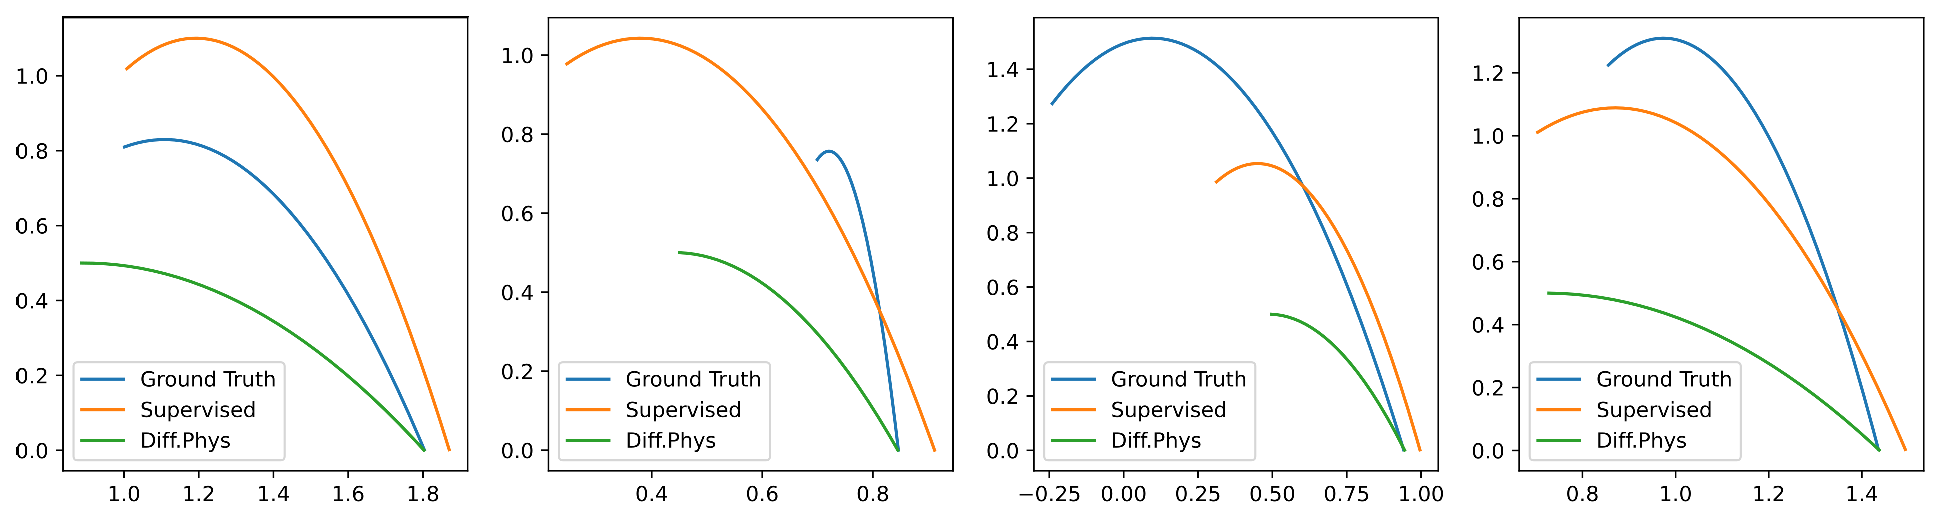
\includegraphics[width=\textwidth]{figures/throwing_results}
  \caption{\todo{Rewrite this.}
    Learning to throw. 
    An example, showcasing an important difference between supervised and
    differentiable physics approaches. Both the supervised and the
    differentiable physics network approximate the function
    $f^{-1}(\vb{x_{final}}): \mathbb{R} \mapsto \mathbb{R}^4$, which is the
    inverse of the function $f(\vb{x}, \vb{y}, \vb{v}, \vb{\alpha})$, mapping
    the final position $\vb{x_{final}}$ of an object being thrown from position
    $(\vb{x}, \vb{y})$, with velocity $\vb{v}$ and angle $\vb{\alpha}$. The same
    network architecture is used, with the weights initialized to the same
    initial values. Both networks have seen the same number of training
    examples, and are using an $L_2$ norm between the point of impact resulting
    from the predicted initial values and the intended position. It is evident
    that the DP network is able to get orders of magnitude closer than the
    supervised network, which has no knowledge of the underlying physical
    system, and it's best guess is to interpolate between the closest data it
    has seen during training, which results in a coarse approximation. Also, as
    the result space to this problem is not unimodal (e.g. it has multiple
    possible right answers), the supervised model is further thrown off, and
    will give values in-between. This means that even if we increase the
    training data, our supervised model can never learn this problem properly.
    (Recreated from
    \url{https://github.com/tum-pbs/PhiFlow/blob/develop/docs/Learn_to_Throw_Tutorial.ipynb})
  }
    \label{fig:learning-to-throw}
\end{figure}

\chapter{Fluid Simulation}

\todo{Write about Fluid Simulation in general, citing the SIGGRAPH course for
the most part + other relevant papers.}

\section{The Laplacian Eigenfunction Method}
\citet{dewitt}

\todo{Write about the eigenfluid algorithm}

\chapter{Results}

\todo{Show the results of our research here}

\chapter{Discussion and Future Work}\label{chapter:discussion}

\todo{Write discussion, assess what we achieved.}

\subsection*{Generalizing to 3D}
All of the introduced method generalize to 3D in a very straightforward way. As
shown by \cite{scalable-eigenfluids}, the Laplacian Eigenfluids technique is
a viable simulation for three dimensional incompressible fluid flow. The
exponential increase of simulation variables is a problem not only in forward
simulations, but especially when computing gradients for optimizing. 

\subsection*{General Improvements to the NN}
After introducing a simple training process, and purposefully keeping our
architecture simple, a number of improvements from the continuously expanding
literature on \ac{DL} and \ac{AI} techniques could be incorporated to improve
our solution.

\subsection*{Improving the Loss Function}
The loss function for the shape transition problem could also be improved in
a number of ways. In our solution, we estimate the trajectory as a linear
interpolation between start and end positions. \

\subsection*{Point Sampling}
In general, estimating functions by sampling discrete points fits into a vast
body of existing literature. The sampling strategies introduced in
section~\ref{section:sampling} could be expanded upon such that advecting the
discrete sample points approximates the natural advection trajectory of the
initial shape as defined by a scalar marker density function.



% Acknowledgements
%----------------------------------------------------------------------------
\chapter*{\koszonetnyilvanitas}\addcontentsline{toc}{chapter}{\koszonetnyilvanitas}
%----------------------------------------------------------------------------

\todo{Write Acknowledgements}


% List of Figures, Tables
%\listoffigures\addcontentsline{toc}{chapter}{\listfigurename}
%\listoftables\addcontentsline{toc}{chapter}{\listtablename}

% Bibliography
\addcontentsline{toc}{chapter}{\bibname}
\bibliography{bib/mybib}

% Appendix
%----------------------------------------------------------------------------
\appendix
%----------------------------------------------------------------------------
\chapter*{\fuggelek}\addcontentsline{toc}{chapter}{\fuggelek}
\setcounter{chapter}{\appendixnumber}
%\setcounter{equation}{0} % a fofejezet-szamlalo az angol ABC 6. betuje (F) lesz
\numberwithin{equation}{section}
\numberwithin{figure}{section}
\numberwithin{lstlisting}{section}
%\numberwithin{tabular}{section}

%----------------------------------------------------------------------------
\section{Precomputation of the Advection Dynamics}
%----------------------------------------------------------------------------




%\label{page:last}
\end{document}
